\documentclass[leno,xcolor=dvipsnames]{beamer}
\usetheme[
    block=fill,         % ブロックに背景をつける
    progressbar=foot,   % 各スライドの下にプログレスバー
    numbering=fraction  % 合計ページ数を表示
]{metropolis}           % Use metropolis theme

\usepackage{luatexja}% 日本語したい
\usepackage[ipaex]{luatexja-preset}% IPAexフォントしたい
\renewcommand{\kanjifamilydefault}{\gtdefault}% 既定をゴシック体に
\makeatletter
\newcommand{\figcaption}[1]{\def\@captype{figure}\caption{#1}}
\newcommand{\tblcaption}[1]{\def\@captype{table}\caption{#1}}
\makeatother

\usepackage{adjustbox}
\usepackage{float}
\usepackage{wrapfig}  % 図の回り込み
\usepackage{blindtext}
\usepackage{booktabs}
\usepackage{multirow}
\usepackage{ascmac}
\usepackage{fancybox}
\usepackage{amsmath}
\usepackage{mathtools}
\usepackage{siunitx}
\usepackage{tikz}
\usetikzlibrary{arrows.meta,bending}
\usepackage{listings}
\lstset{
    frame=single,
    basicstyle=\tiny\ttfamily,
    tabsize=4
}

\title{進捗報告}
\date{\today}
\author{水野泰旭}
\institute{弘前大学理工学部電子情報工学科4年}
\begin{document}
  \maketitle

  \begin{frame}[plain]{目次}
    \tableofcontents
  \end{frame}

  \begin{frame}[plain]
    \section{Macro-F1スコア}
  \end{frame}

  \begin{frame}{macro-F1スコアの計算}
    混同行列を用いて計算していく。
    \begin{figure}[H]
      \centering  
      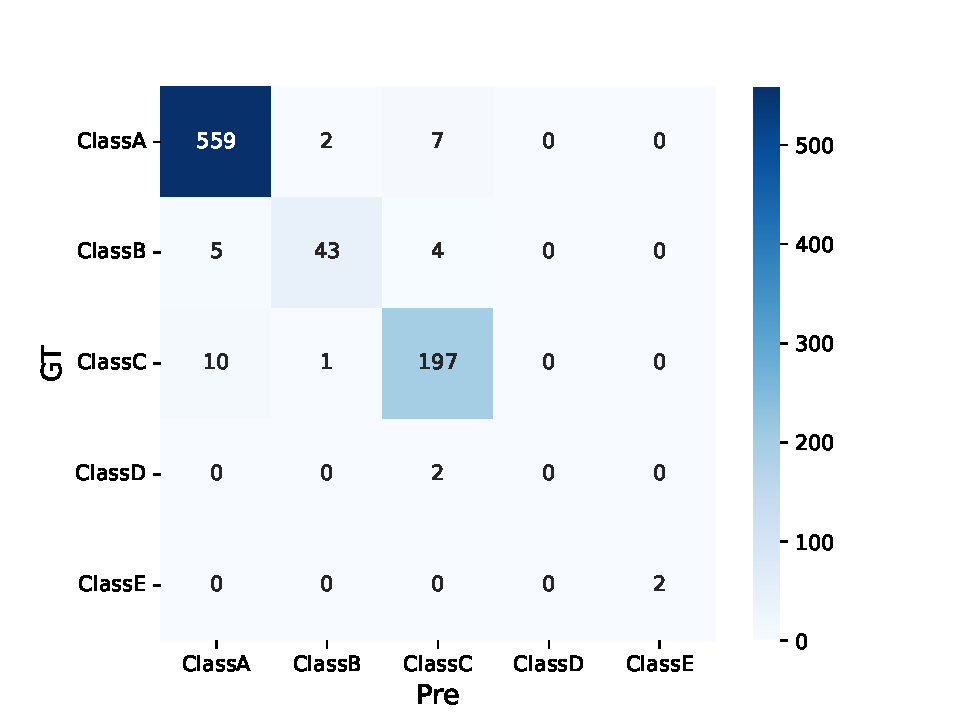
\includegraphics[keepaspectratio,scale=0.5]{images/deepimfam_confusion_matrix_cnt.pdf}
    \end{figure}
  \end{frame}

  \begin{frame}{macro-F1スコアのClassAの場合}
    \begin{minipage}[t]{.48\textwidth}
      \begin{table}
        \caption{Class A} \label{tb:ClassA}
        \begin{adjustbox}{width=\columnwidth, center}
          \begin{tabular}{ccll}
            \toprule
            \multicolumn{2}{c}{} & \multicolumn{2}{c}{予測値} \\ \cline{3-4}
            & & 陽性 & 陰性 \\
            \midrule
            \multirow{2}{*}{正解率} & 陽性 & TP=559 & FN=9 \\
            & 陰性 & FP=15 & TN=249 \\
            \bottomrule
          \end{tabular}
        \end{adjustbox}
      \end{table}
    \end{minipage}\hfill
    \begin{minipage}[t]{.48\textwidth}
      \begin{figure}
        \centering
        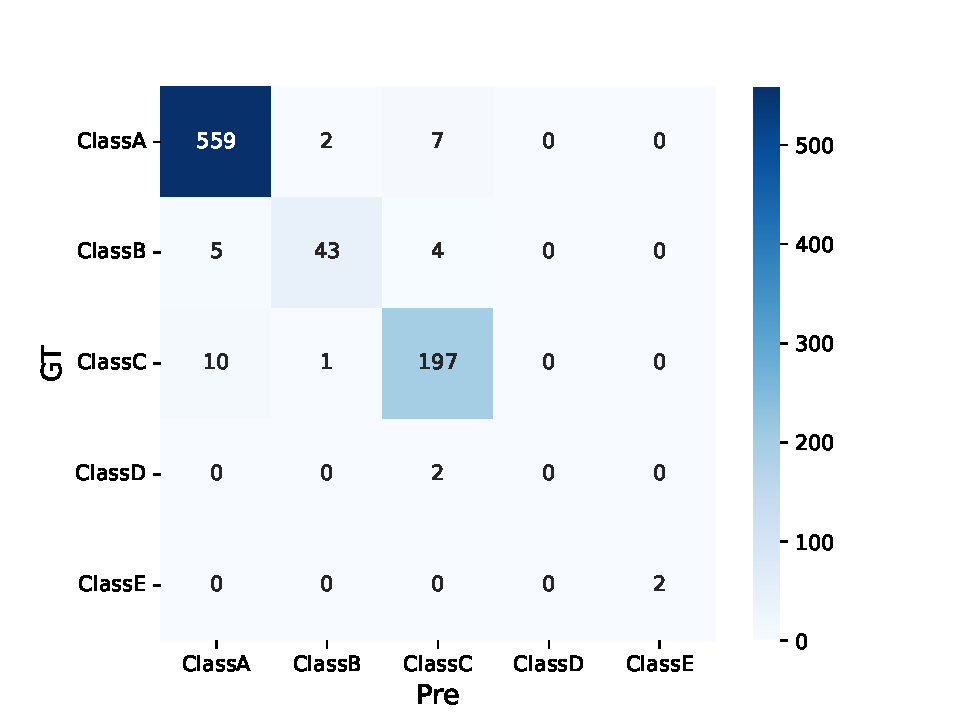
\includegraphics[keepaspectratio,scale=0.3]{images/deepimfam_confusion_matrix_cnt.pdf}
      \end{figure}
    \end{minipage}
    \begin{align*}
      \mathrm{Accuracy} &= 0.971153846153846 \\
      \mathrm{Precision} &= 0.9738675958188153 \\
      \mathrm{Recall} &= 0.984154929577465 \\
      \mathrm{macro-F1} &= 0.978984238178634
    \end{align*}
  \end{frame}

  \begin{frame}
    \begin{table}[H]
      \centering
      \caption{クラスごとのMacro-F1の計算} \label{tb:macro-F1}
      \begin{tabular}{ccccc}
        \toprule
        Class & Accuracy & Precision & Recall & Macro-F1 \\
        \midrule
        A & 0.97115 & 0.97386 & 0.98415 & 0.97898 \\
        B & 0.98557 & 0.93478 & 0.82692 & 0.87755 \\
        C & 0.97115 & 0.93809 & 0.94711 & 0.94258 \\
        D & 0.99759 & - & 0.0000 & - \\
        E & 1.00000 & 1.0000 & 1.0000 & 1.0000 \\
        \midrule
        Average\footnote{平均値を出すためクラスDのPrecisionとMacro-F1の値を最小値である0として計算} & 0.98509 & 0.76934 & 0.75163 & 0.75982 \\
        \bottomrule
      \end{tabular}
    \end{table}
  \end{frame}

  \begin{frame}{考察}
    \begin{itemize}
      \item \href{https://scikit-learn.org/stable/modules/generated/sklearn.metrics.f1_score.html}{sklearn}を用いてMacro-F1を計算すると0.75982が出力され、計算結果が正しいことがわかった
      \item クラスの個数が大きく異なるので、それぞれのクラスのFスコアの平均を取るの正確に評価できない
      \begin{itemize}
        \item \href{https://www.ibm.com/docs/en/cloud-paks/cp-data/3.5.0?topic=overview-weighted-f1-measure}{$\mathrm{F}_{\beta}$}を用いる \mbox{}\\ slearnを用いて0.9612417267002779
        \item micro-F1
      \end{itemize}
    \end{itemize}
  \end{frame}

  \begin{frame}
    \section{Micro-F1}
  \end{frame}
  
  \begin{frame}{\href{https://ebi-works.com/macrof1/\#outline__1_2}{Micro-F1}}
    \begin{align*}
      \mathrm{micro\text{-}F1} &= \frac{2}{\frac{1}{\mathrm{Precision}_{\mathrm{total}}} + \frac{1}{\mathrm{Recall}_{\mathrm{total}}}} \\
      \mathrm{Precision}_{\mathrm{total}} &= \frac{\sum TP}{\sum TP + \sum FP} \\
      \mathrm{Recall}_{\mathrm{total}} &= \frac{\sum TP}{\sum TP + \sum FN}
    \end{align*}
    計算した結果、すべて同じ数値になった。
  \end{frame}

\end{document}